\section{Spline Fitting Method}
\label{Spline_1}

In this paper there are 2 methods of fusing IMU data and Monocular camera. First of which is spline fitting using scale factor with the data of IMU and Monocular camera. Depending on the reliability of the data from both sources to estimate distance.So here we did simulation of whole system with arbitrary value of data considering linear moment of robot with noisy data. These simulations can be seen in result section. With the matlab code. So initially theory behind curve fitting is explained to have a algebraic background of types of curve fitting and their applications.We use spline in curve fitting because we get discrete data from sensors and camera but tracing spline helps for interpolation and extrapolation to have continuous high probability data of path.

Spline is fitted on the data points which is output of sensor in our case. Spline fitting also helps in reducing error due to noise. For Improving accuracy we can increase number of spline but this will also result into increase in computation. So we have to trade off between accuracy and computation.
Spline fitting is useful to give smooth curve .N degree spline may has N-1 curves in its shape. So if spline has X3 term that means it can have 2 curves in its spline.Ideal method to cover n points in a plan is by tracing nth order spline which will result into zero error. So spline will pass through all the points and will have a general equation as

\begin{equation}
\ A_{0} +A_{1}X +A_{2}X^{2}+A_{3}X^{3} + ... + A_{n}X^{n} = Y
\end{equation} 

This problem then converts in simple Ax = B form. we can get values of n terms by plugging in n points values.

Where

\begin{equation}
A = 
\begin{pmatrix}
  1 & X_{1} & X_{1}^{2} & \cdots & X_{1}^{n} \\
  1 & X_{2} & X_{2}^{2} & \cdots & X_{2}^{n} \\
  1 & X_{3} & X_{3}^{2} & \cdots & X_{3}^{n} \\
  : & :     &     :     & \cdots &    :      \\
  1 & X_{n} & X_{n}^{2} & \cdots & X_{n}^{n} \\
 \end{pmatrix}
B = 
\begin{pmatrix}
  A_{0} \\
  A_{1} \\
  A_{2} \\
  : 	\\
  A_{n} \\
 \end{pmatrix}
 C = 
\begin{pmatrix}
  Y_{0} \\
  Y_{1} \\
  Y_{2} \\
  : 	\\
  Y_{n} \\
 \end{pmatrix}
\end{equation}

But for practical applications we use other methods and do not plot n degree spline as it is computationally expensive .Secondly if there is more noise in system it will give wrong results. 
For practical application there are 3 kinds of spline fitting according to the application:-

\subsection{Types of curve fitting}
\subsubsection{Maximum error}
This is the method where spline is fit in a way where the point with maximum error is reduced and curve move towards the outlier point. If there exist in order to reduce maximum error of a point. This on the other hand results into

\begin{figure}[!htb]
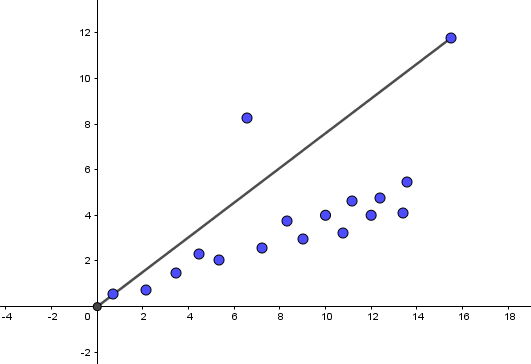
\includegraphics[width=\textwidth]{./figures/Maxerror.PNG}
\caption{Curve Fitting with Maximum error }
\end{figure}

\begin{equation}
E(f)=|max (f(xi)-yi)|  where i goes from 1 to left n
\end{equation}

Actually due to one outlier here line shifted in order to reduce maximum error. So this is not reliable process but is easy to compute.

\subsubsection{Average error}
This method is used to minimize average and fit the spline with minimum error conditions.

\begin{figure}[!htb]
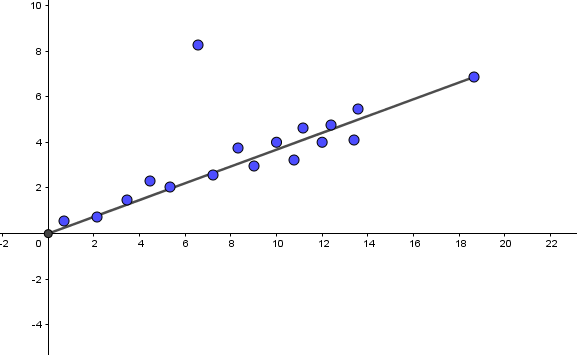
\includegraphics[width=\textwidth]{./figures/average.PNG}
\caption{Curve Fitting with Average error }
\end{figure}

\begin{equation}
E(f)=\frac{1}{n}*\Sigma|f(x_k)-Y_k| 
\end{equation}

Actually due to one outlier here line shifted in order to reduce maximum error. So this is not reliable process but is easy to compute.

\subsubsection{RMS (Least square method)}
This is the most efficient method to minimize the error this is also called as least square method.
Hence this is mostly used in curve fitting.
We have also created an algorithm with the help of same type of curve fitting.

\begin{figure}[!htb]
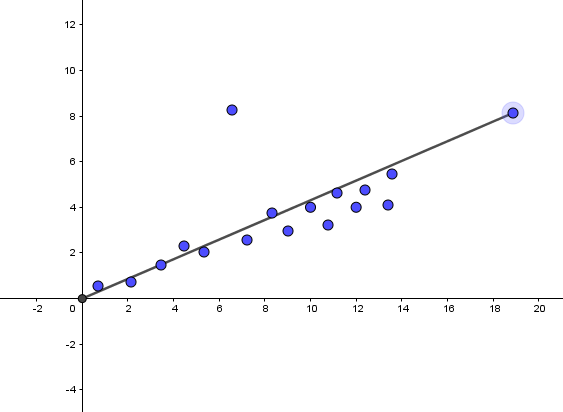
\includegraphics[width=\textwidth]{./figures/RMS.PNG}
\caption{Curve Fitting with RMS error }
\end{figure}

\begin{equation}
E(f)={\lbrace\frac{1}{n}*\Sigma|f(x_k)-Y_k|\rbrace}^\frac{1}{2} 
\end{equation}

\subsection{IMU Reading}
As we don’t have real IMU lets simulate virtual readings for this we took X, Y, Z as a function on time 

\begin{equation}
\label{For_x}
X_1=A_y t^2+B_y t +C_x
\end{equation}

\begin{equation}
Y_1=A_y t^2+B_y t +C_y
\end{equation}

\begin{equation}
Z_1=A_z t^2+B_z t +C_z
\end{equation}

With this treatment we will add some random noise to all the terms so that the data can be similar to what we obtain form IMU.

\begin{equation}
noise=A*(rand(1,n)-0.5)
\end{equation}

So our noise will range from -A/2 to A/2.
As function is rand() so it will change for every point.

\begin{equation}
X=X_1+noise
\end{equation}

\begin{equation}
Y=Y_1+noise
\end{equation}

\begin{equation}
Z=Z_1+noise
\end{equation}
We also took some random points of camera pose. And provided our system with data set.
Proof of Least square method in our case:
Let’s consider optimization of X first.
 
From equation \eqref{For_x} we have

Here $A$, $B$, $C$ are known
We have data set of X with respect to t
To calculate error in RMS we have
 
\begin{equation} 
 Error_x={\lbrace\displaystyle\sum_{i=1}^{n}(|X_i-(A_xt_i^2+B_x t_i +C_x)|)^2\rbrace}^\frac{1}{2} 
\end{equation}


When we differentiate some quantity and equate it to zero it goes to either minima or maxima
And if double derivative is positive it goes to minima.

So in this case if we take partial derivatives of error with respect to Ax , Bx , Cx

\begin{equation} 
 \frac{\partial Error_x}{\partial A_x} = {\lbrace\displaystyle\sum_{i=1}^{n}2(|X_i-(A_xt_i^2+B_x t_i +C_x)|)\rbrace}({-t_i^2})
\end{equation}

\begin{equation} 
\displaystyle\sum_{i=1}^{n}(|{-t_i^2}X_i+(A_x t_i^4+B_x t_i^3+C_x t_i^2)|) = 0
\end{equation}

\begin{equation} 
 \frac{\partial Error_x}{\partial B_x} = {\lbrace\displaystyle\sum_{i=1}^{n}2(|X_i-(A_xt_i^2+B_x t_i +C_x)|)\rbrace}({-t_i})
\end{equation}

\begin{equation} 
\displaystyle\sum_{i=1}^{n}(|{-t_i}X_i+(A_x t_i^3+B_x t_i^2+C_x t_i^1)|) = 0
\end{equation}

\begin{equation} 
 \frac{\partial Error_x}{\partial C_x} = {\lbrace\displaystyle\sum_{i=1}^{n}2(|X_i-(A_xt_i^2+B_x t_i +C_x)|)\rbrace}({-1})
\end{equation}

\begin{equation} 
\displaystyle\sum_{i=1}^{n}(|{-1}X_i+(A_x t_i^2+B_x t_i+C_x)|) = 0
\end{equation}

So we can compute matrix in such a way that the problem changes to 

Ax=B

Where, 

\begin{equation}
A = 
\begin{pmatrix}
  \Sigma t^4 & \Sigma t^3 & \Sigma t^2\\
  \Sigma t^3 & \Sigma t^2 & \Sigma t\\
  \Sigma t^2 & \Sigma t & \Sigma 1\\
 \end{pmatrix}
B = 
\begin{pmatrix}
  A_x \\
  B_x \\
  C_x \\
 \end{pmatrix}
 C = 
\begin{pmatrix}
  \Sigma X_i t ^2 \\
  \Sigma X_i t \\
  \Sigma X_i \\
 \end{pmatrix}
\end{equation}

From this equation we can calculate X matrix.Similarly,We can get X matrix of Y and Z axis.

\begin{equation}
A = 
\begin{pmatrix}
  \Sigma t^4 & \Sigma t^3 & \Sigma t^2\\
  \Sigma t^3 & \Sigma t^2 & \Sigma t\\
  \Sigma t^2 & \Sigma t & \Sigma 1\\
 \end{pmatrix}
B = 
\begin{pmatrix}
  A_y \\
  B_y \\
  C_y \\
 \end{pmatrix}
 C = 
\begin{pmatrix}
  \Sigma Y_i t ^2 \\
  \Sigma Y_i t \\
  \Sigma Y_i \\
 \end{pmatrix}
\end{equation}

\begin{equation}
A = 
\begin{pmatrix}
  \Sigma t^4 & \Sigma t^3 & \Sigma t^2\\
  \Sigma t^3 & \Sigma t^2 & \Sigma t\\
  \Sigma t^2 & \Sigma t & \Sigma 1\\
 \end{pmatrix}
B = 
\begin{pmatrix}
  A_z \\
  B_z \\
  C_z \\
 \end{pmatrix}
 C = 
\begin{pmatrix}
  \Sigma Z_i t ^2 \\
  \Sigma Z_i t \\
  \Sigma Z_i \\
 \end{pmatrix}
\end{equation}

By this treatment we converted given points into equation with least square method here we used condition of 

\begin{equation}
min
\begin{pmatrix}
  A_x t^2 + B_x t + C_x -\lambda_i X_c \\
  A_y t^2 + B_y t + C_y -\lambda_i Y_c \\
  A_z t^2 + B_z t + C_z -\lambda_i Z_c \\
 \end{pmatrix}^2
 \end{equation}
 
 Here in this formula we have different value of  for different spline according to accuracy of camera data and IMU reading.

\subsection{Results}
 
 In our case we simulated the results and found following outputs.
Plotting the second order curve for given data of IMU with just least square method. We get

\begin{figure}[!htb]
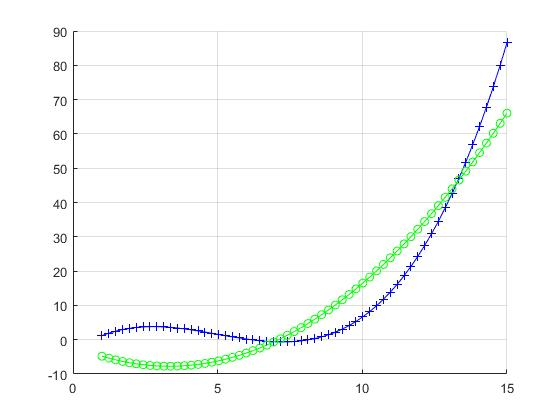
\includegraphics[width=\textwidth]{./figures/lsm.jpg}
\caption{In this case Blue is actual curve traced by IMU this are points with noise.And green is plotted curve. With least square method.}
\end{figure}

Then according to the paper we fused data of camera and IMU so we get following graph.

\begin{figure}[!htb]
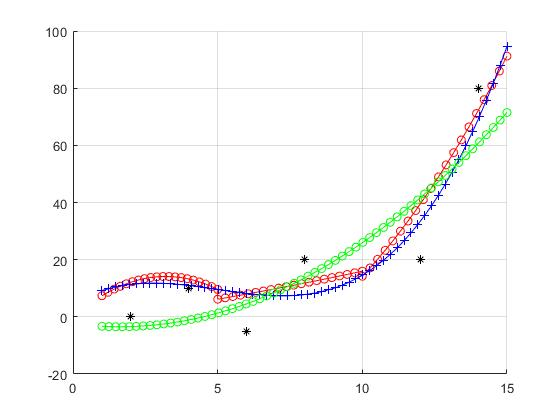
\includegraphics[width=\textwidth]{./figures/AllOutput.jpg}
\caption{Multiple spline fit}
\label{fig:multipleSpline}
\end{figure}

In Figure~\ref{fig:multipleSpline} we have 3 curved fitted as shown as red which gives better results and it also uses data of camera shown with black dots. So here according to the above formula scale factor of different section is different it is according to the quality of reading by camera.
For example, in our case 
\begin{equation}
\lambda_1=0.5 ,\lambda_2=0.5 ,\lambda_3=0.1
\end{equation}

In 3rd section camera readings were not accurate so taken into smaller scalar value. This camera data further improved the result. And we get minimum error and good fit. With the given spline fitting method.

So if we look into different of error with traditional Least square method with Jung and Taylor method. It gives good results. Almost we get the same curve.

\begin{figure}[!htb]
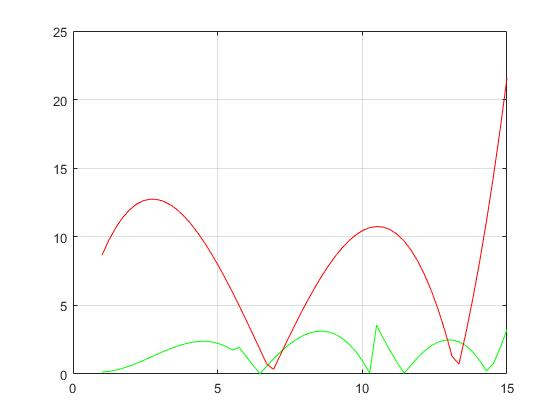
\includegraphics[width=\textwidth]{./figures/ErrorC.jpg}
\caption{A. Red curve for method with one curve and least square method. 
B. Green curve is using the given method by Jung and Taylor.}
\label{fig:errorc1}
\end{figure}

The graph in Figure~\ref{fig:errorc1} has error comparison with and without Jung and Taylor method of split curve fitting and scaling camera input.
So it is better to follow the given first method in the paper. It results into considerable reduction in error which is clearly seen in graph.
  